\documentclass{beamer}
\usefonttheme[onlylarge]{structuresmallcapsserif}
\usefonttheme[onlysmall]{structurebold}
\usetheme{Warsaw}
\setbeamercovered{transparent}
\usepackage{fancybox,color,tcolorbox}
\usepackage{verbatim}
\usepackage[english,spanish,activeacute]{babel}
%\usepackage[latin1]{inputenc}
\usepackage{inputenc}
\usepackage{latexsym}
\usepackage{amsmath}
\usepackage{graphicx} % Allows including images
\usepackage{booktabs}
\usepackage{amssymb}
\usepackage{multimedia}
\usepackage{pifont,pgfcore}
\usepackage{tcolorbox}
\usepackage{animate}
\usepackage{ucs}

\newtheorem*{Theorem*}{Teorema}
\newtheorem*{Definition*}{Definici'on}
\newtheorem*{Example*}{Ejemplo}

\title[Perez Marquez]{Moogle!}
\author[Pedro Dennis]{Pedro Dennis Perez Marquez}
\date{\today}

\begin{document}
%-----Redefiniendo colores----------%
\definecolor{myred}{RGB}{200,0,0}
\definecolor{myvio}{RGB}{100,200,100}
\definecolor{mygreen}{RGB}{0,150,150}
\setbeamercolor{title}{fg=myred}
\setbeamercolor{frametitle}{bg=myvio, fg=white}
\setbeamercolor{structure}{fg=mygreen}
\begin{frame}
 \titlepage
  \begin{center}
    \colorbox{black}{\textbf{\begin{large}\textcolor{white}{Buscador Moogle.}\end{large}}}\\\ \\
    \scriptsize \textbf{\textcolor{black}{Facultad Matem\'atica Computaci\'on}}\\
    \textbf{\textcolor{green}{Universidad de La Habana}}
  \end{center}
\end{frame}
%-----------------------------------------------

%-------------------------------------------------
\begin{frame}
	\frametitle{Temas a tratar} 
	\tableofcontents 
\end{frame}
%------------------------------------

%-------------------------------------
\section{Introducci\'on}
\begin{frame}
\begin{minipage}{10cm}
	 Moogle! es una innovadora aplicación diseñada para buscar de manera inteligente un texto específico en un conjunto de documentos. Esta aplicación web ha sido desarrollada con tecnología .NET Core 6.0, utilizando Blazor como framework web para la interfaz gráfica. Moogle! se divide en dos componentes principales: MoogleServer, que es un servidor web capaz de renderizar la interfaz gráfica y ofrecer los resultados; y MoogleEngine, una biblioteca de clases que implementa la lógica del algoritmo de búsqueda. 
\end{minipage}
\end{frame}

\section{Formulaci\'on matem\'atica}

\begin{frame}
\frametitle{Modelo matemático}
\begin{minipage}{10cm}
	La formulación utilizada es TF IDF \\
	\begin{equation}\label{eq:general}
			\begin{cases}
			TF = n/N   \\
			IDF = log(1+D/d)
			\end{cases}
	\end{equation} 
	La variable $''n''$ representa la cantidad de apariciones de una palabra en un documento y $''N''$ representa la cantidad de palabras del documento. En el caso del IDF la variable $''D''$ representa la cantidad de documentos existentes y $''d''$ la cantidad de documentos que contienen la palabra en cuestion. \\
	De esta forma al realizar la multiplicacion del TF y el IDF, obtendriamos la relvancia de esa palabra en esos documentos.
\end{minipage}

\end{frame}	

\begin{frame}
	% \frametitle{Modelo matemático}
	\begin{minipage}{10 cm}
		Una vez calculado el TDIDF de todos los documentos se procede de la siguiente forma:
		\begin{itemize}
			\item Si $TFIDF=0$, el documento no tendria relevancia y no se moestraria.
			equilibrio.
			\item Si $TFIDF > 0$, el documento se compararia con otros y se mostrarian en orden descendente.
		\end{itemize}
	Una ves hecho esto los documentos quedan organizados por orden de relevancia.
	\end{minipage}
\end{frame}

\begin{frame}
	% \frametitle{Modelo matemático}
	\begin{minipage}{10 cm}
La distancia de Levenshtein, también conocida como distancia de edición o distancia entre palabras, es una métrica ampliamente utilizada en teoría de la información y ciencias de la computación. Se define como el número mínimo de operaciones necesarias para transformar una cadena de caracteres en otra, donde una operación puede ser una inserción, eliminación o sustitución de un carácter. Esta distancia es especialmente útil en programas que determinan la similitud entre dos cadenas de caracteres, como los correctores ortográficos. La distancia de Levenshtein lleva el nombre del científico ruso Vladimir Levenshtein, quien la propuso por primera vez en 1965. Con su amplia aplicación en la informática, esta métrica ha demostrado ser una herramienta valiosa para la comparación y análisis de cadenas de caracteres.
		\begin{itemize}
			\item casa cala(sustitucion 's' por 'l')
			\item cala calla(insercion de 'l' ente 'l' y 'a')
                   \item  calla calle(sustitucion de 'a' por 'e')
		\end{itemize}
	\end{minipage}
\end{frame}

\begin{figure}[h]
    \centering
	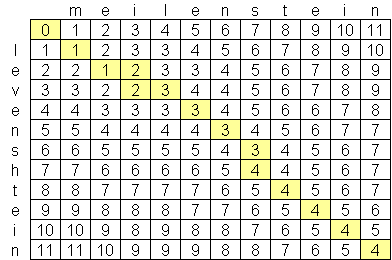
\includegraphics[width=0.68\textwidth]{anexo1.png}
    \caption{Anexo1: Distancia de Lvenshtein}
    \label{img:3}
\end{figure}







\begin{frame}
	\frametitle{Funcionalidades del Moogle}
	\begin{minipage}{10 cm}
		Durante la ejecución del programa, se realiza una extracción inicial de los archivos de texto ubicados en la ruta asignada. Estos textos se procesan y se calcula el TD, IDF y TF-IDF para cada palabra distinta presente en el documento. Este proceso garantiza que, una vez que toda la información ha sido procesada, las búsquedas se realicen de manera más rápida y eficiente. Al realizar una búsqueda, el programa la procesa y la almacena en un array, que, a su vez, se multiplica por la matriz que contiene los TF-IDF de cada texto. Se aplican los cambios correspondientes en relación con los símbolos y, de esta manera, se obtiene el puntaje de cada texto. En el caso de que una palabra de la búsqueda no se encuentre en el conjunto de textos, Moogle! le proporcionará sugerencias relevantes. De manera similar, si se cometió un error de ortografía en la búsqueda, Moogle! detectará automáticamente la palabra correcta y la mostrará en los resultados.
Cuenta a su vez con caracteres especiales de busqueda: ('!', '\^{}', '~', '*')
	\end{minipage}
\end{frame}





\begin{frame}
	\frametitle{Caracteres especiales}
	\begin{minipage}{10cm}
	\begin{alertblock}{'!'}
		 Delante de una palabra devuelve txt donde esta palabra no puede aparecer.
	\end{alertblock}
	\begin{alertblock}{'\^{}'}
		Delante de una palabra devuelve txt donde esa palabra tiene que aprecer obligatoriamente.
	\end{alertblock}

      \begin{alertblock}{'*'}
            Delante de una palabra, le da a esta palabra mas relevancia en la busqueda. 
      \end{alertblock} 
	\end{minipage}
\end{frame}




%----------------------------------
\section{Conclusiones}

\begin{frame}
	\frametitle{Conclusiones}
	\begin{minipage}{10cm}
		En resumen, Moogle! es un buscador de archivos de texto (.txt) que utiliza un modelo vectorial basado en TF-IDF. Además, incorpora algoritmos como la distancia de Levenshtein para mejorar la eficiencia de la búsqueda. En general, Moogle! es un proyecto altamente eficiente que ofrece una solución efectiva para la búsqueda de información en archivos de texto.
	\end{minipage}
\end{frame}


\end{document}


